\documentclass[
]{beamer}

\usepackage[english]{babel}
\usepackage[utf8]{inputenc}
\usepackage[T1]{fontenc}
\usepackage{lmodern}
\usepackage{csquotes}
\usepackage{expl3,biblatex}
\addbibresource{sources.bib}
\usepackage{booktabs}
\usetheme[
  workplace=fi,
  fonts=none,
]{MU}
\setbeamerfont{footnote}{size=\scriptsize}
\usepackage{textalpha}
\usepackage{subfigure}
\makeatletter
\renewcommand{\@thesubfigure}{\space}
\renewcommand{\thesubfigure}{}
\makeatother
\usepackage{wrapfig}
\usepackage{tikz}
\usepackage{appendixnumberbeamer}

\title[Visualisation and Annotation of VolSeg Data in Mol*]{Lightweight Visualisation and Annotation of Volumetric and Segmentation Data in Mol*}
\subtitle[Master's Thesis Defense]{Master's Thesis Defense}
\author[D. Tichý]{Author:\hspace{0.63em}Bc. Dominik Tichý\texorpdfstring{\\}{, }Advisor: RNDr. Tomáš Raček, Ph.D.}
\institute[FI MU]{Faculty of Informatics, Masaryk University}
\date{January 30, 2026}
\subject{Presentation Subject}
\keywords{Mol*, Mol* VS, MolViewSpec, MolViewStories, volumetric data, segmentations, visualization, bioinformatics}

\begin{document}

\begin{frame}[plain,noframenumbering]
\maketitle
\end{frame}

\begin{frame}{Motivation}
  \begin{itemize}
    \item Rapid growth of microscopy data (e.g., Cryo-EM, Cryo-ET) \footfullcite{kuhlbrandt2014resolution}
    \item Critical in structural biology and drug design (e.g., SARS-CoV-2 spike protein characterization) \footfullcite {wrapp2020covid}
    \item Need for a web-based tool to visualize and annotate
  \end{itemize}
\end{frame}

\begin{frame}{Theory}{Volumes}
  \begin{itemize}
    \item Raw measured data from microscopes
    \item 3D scalar grids representing electron density or potential
    \item Isovalue is a threshold used to extract a 3D surface
  \end{itemize}
  \begin{figure}
    \centering
    \subfigure[$v=0.05$]{\includegraphics[width=0.3\textwidth,keepaspectratio]{images/1832-005.png}}
    \subfigure[$v=0.15$]{\includegraphics[width=0.3\textwidth,keepaspectratio]{images/1832-015.png}}
    \subfigure[$v=0.30$]{\includegraphics[width=0.3\textwidth,keepaspectratio]{images/1832-03.png}}
  \end{figure}  
\end{frame}

\begin{frame}{Theory}{Segmentations}
  \begin{itemize}
    \item Gives the raw volumetric data biological meaning
    \item Convert continuous intensity signals into discrete objects
    \item Lattices, meshes, geometric primitives
  \end{itemize}
  \begin{figure}
    \includegraphics[height=0.6\textheight,keepaspectratio]{./images/Gemini_Generated_Image_97q74g97q74g97q7.png}
  \end{figure}
\end{frame}

\begin{frame}{Mol*}
  \begin{itemize}
    \item Mol* platform \footfullcite{Sehnal2021Molstar}
    \item Mol* Volumes and Segmentation (Mol* VS) \footfullcite{Chareshneu2024Volseg}
    \begin{itemize}
      \item Difficult to use and maintain
      \item Lacks interoperability
      \item Siloed data formats
    \end{itemize}
    \item MolViewSpec (MVS) \footfullcite{Midlik2025MolViewSpec}
    \begin{itemize}
      \item Declarative standard
      \item Describes ``what'' the scene looks like, not ``how'' to build it
    \end{itemize}
  \end{itemize}
\end{frame}

\begin{frame}{Mol*}{Formats}
  \begin{itemize}
    \item compare CVSX and MVSX side by side
  \end{itemize}
\end{frame}

\begin{frame}{Goals}
  \begin{alertblock}{Thesis Objective}
    Show that MolViewSpec can be used to visualize and annotate volumetric and segmentation data in Mol*
  \end{alertblock}
  \begin{itemize}
    \item \textbf{Goal 1:} Create a conversion library (CVSX $\rightarrow$ MVSX)
    \item \textbf{Goal 2:} Web application for non-technical users
  \end{itemize}
\end{frame}

\begin{frame}{Conversion Library}
  \begin{itemize}
    \item \textbf{Extract:} Read CVSX file contents
    \item \textbf{Transform:} Convert CVSX primitives to MVSX analogues
    \item \textbf{Load:} Serialize to MVS file formats
  \end{itemize}
  \begin{figure}
    \includegraphics[width=1\textwidth,keepaspectratio]{./images/etl-overview.pdf}
  \end{figure}
\end{frame}

\begin{frame}{Conversion Library --- Implementation}{Volumetric Data}
  \begin{figure}
    \centering
    \includegraphics[width=1\textwidth,keepaspectratio]{./images/volume.pdf}
  \end{figure}
\end{frame}

\begin{frame}{Conversion Library --- Implementation}{Lattice Segmentation}
  \begin{figure}
    \centering
    \includegraphics[width=1\textwidth,keepaspectratio]{./images/lattice.pdf}
  \end{figure}
\end{frame}

\begin{frame}{Conversion Library --- Implementation}{Geometric \& Mesh Segmentation}
  \begin{figure}
    \centering
    \includegraphics[width=1\textwidth,keepaspectratio]{./images/geo-mesh.pdf}
  \end{figure}
\end{frame}

\begin{frame}{Conversion Library --- Results}
  \textbf{Visual Fidelity:}
  \begin{itemize}
    \item Verified on 14 diverse datasets from EMDB, IDR, EMPIAR
  \end{itemize}
  \begin{table}[htbp]
    \centering
    \resizebox{\textwidth}{!}{
    \begin{tabular}{l r@{${}\times{}$}r@{${}\times{}$}l lrr}
      \toprule
      \textbf{Dataset ID} & \multicolumn{3}{c}{\textbf{Image dimensions (XYZ)}} & \textbf{Seg. type} & \textbf{Seg. count} & \textbf{Size (MB)} \\
      \midrule
      \href{https://www.ebi.ac.uk/emdb/EMD-1832}{EMD-1832} & 64 & 64 & 64 & Lattice & 1 & 0.09 \\
      \href{https://www.ebi.ac.uk/emdb/EMD-1273}{EMD-1273} & 2048 & 2048 & 76 & Lattice & 5 & 39.78 \\
      \href{https://www.ebi.ac.uk/emdb/EMD-19111}{EMD-19111} & 440 & 440 & 440 & - & - & 12.15 \\
      \href{https://idr.openmicroscopy.org/webclient/img_detail/6001240}{IDR-6001240} & 271 & 275 & 236 & Lattice & 1 & 40.66 \\
      \href{https://idr.openmicroscopy.org/webclient/img_detail/6001247}{IDR-6001247} & 253 & 210 & 257 & Lattice & 1 & 35.43 \\
      \href{https://idr.openmicroscopy.org/webclient/img_detail/13457537}{IDR-13457537} & 198 & 223 & 12 & Lattice & 1 & 28.03 \\
      \href{https://idr.openmicroscopy.org/webclient/img_detail/5514375}{IDR-5514375} & 256 & 256 & 31 & Lattice & 2 & 493.08 \\
      \href{https://idr.openmicroscopy.org/webclient/img_detail/5025551}{IDR-5025551} & 2702 & 2700 & 1 & - & - & 65.92 \\
      \href{https://idr.openmicroscopy.org/webclient/img_detail/5025552}{IDR-5025552} & 2701 & 2701 & 64 & - & - & 63.29 \\
      \href{https://idr.openmicroscopy.org/webclient/img_detail/5025553}{IDR-5025553} & 2500 & 2500 & 64 & - & - & 96.63 \\
      \href{https://www.ebi.ac.uk/empiar/EMPIAR-10070}{EMPIAR-10070} & 1675 & 1595 & 291 & Mesh & 1 & 56.30 \\
      \href{https://www.ebi.ac.uk/empiar/EMPIAR-11756}{EMPIAR-11756} & 1024 & 1024 & 512 & Geometric & 1164 & 3.93 \\
      \href{https://cryoetdataportal.czscience.com/runs/17803}{CUSTOM-19420} & 1260 & 1260 & 368 & - & - & 32.22 \\
      \href{https://docs.openmicroscopy.org/ome-model/5.6.3/ome-tiff/data.html}{CUSTOM-TUBHISWT} & 512 & 512 & 10 & - & - & 106.10 \\
      \bottomrule
    \end{tabular}
    }
  \end{table}
\end{frame}

\begin{frame}{Conversion Library --- Results}
  \textbf{File Size:}
  \begin{itemize}
    \item Minimal overhead ($<5\%$) for most mappings
    \item Except for lattice-to-mesh conversion ($10-50\%$)
  \end{itemize}
  
  \textbf{Improvements:}
  \begin{itemize}
    \item Fixed missing volumes, restored color annotations
    \item Corrected author-defined contour levels
    \item Proper isosurface capping
  \end{itemize}
\end{frame}

\begin{frame}{Conversion Library --- Improvements}
  \begin{figure}
    \centering
    \subfigure[CVSX]{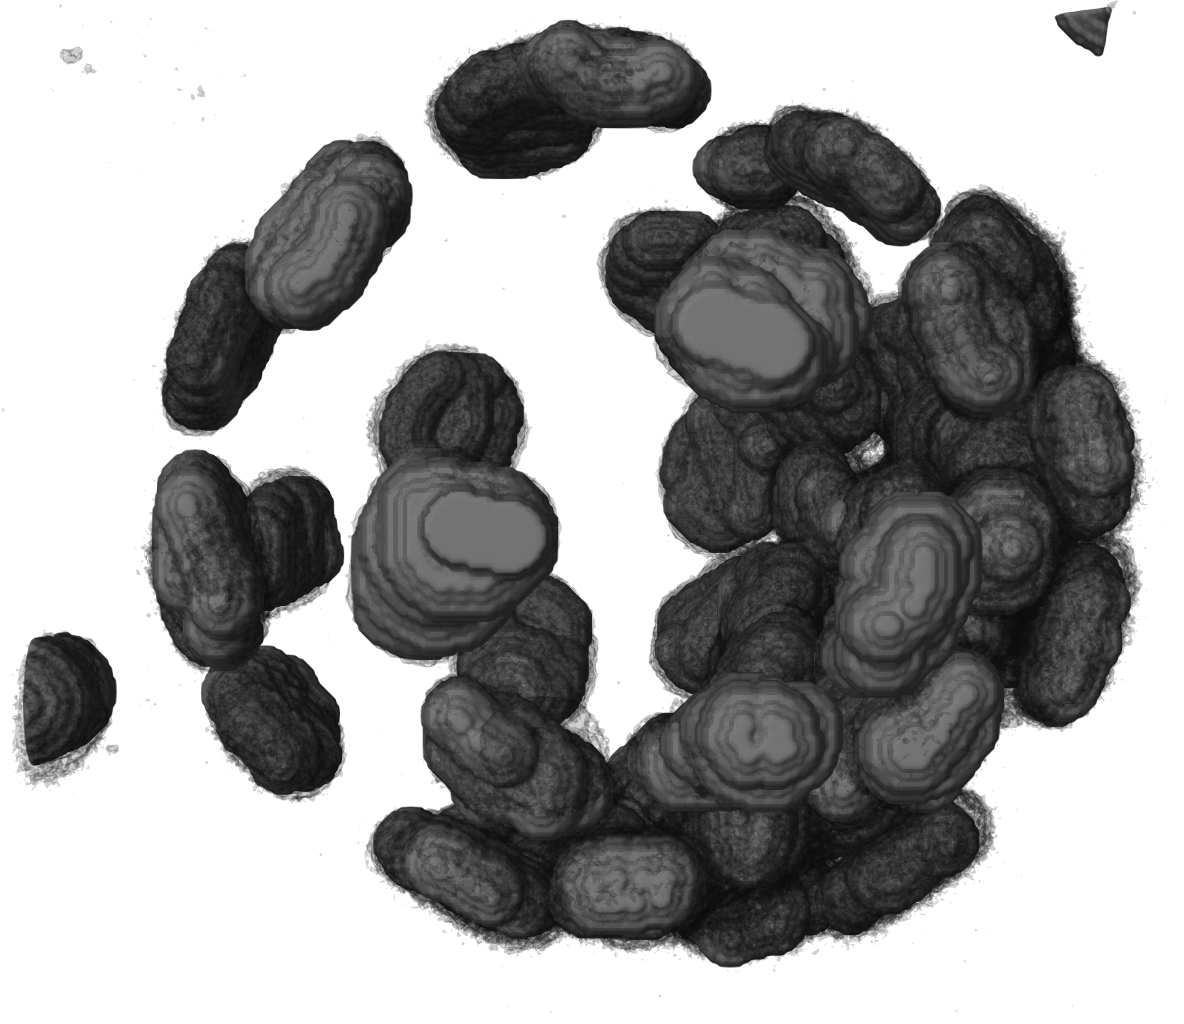
\includegraphics[height=0.5\textheight,keepaspectratio]{images/idr-6001240-cvsx.png}}
    \hspace{1cm}
    \subfigure[MVSX]{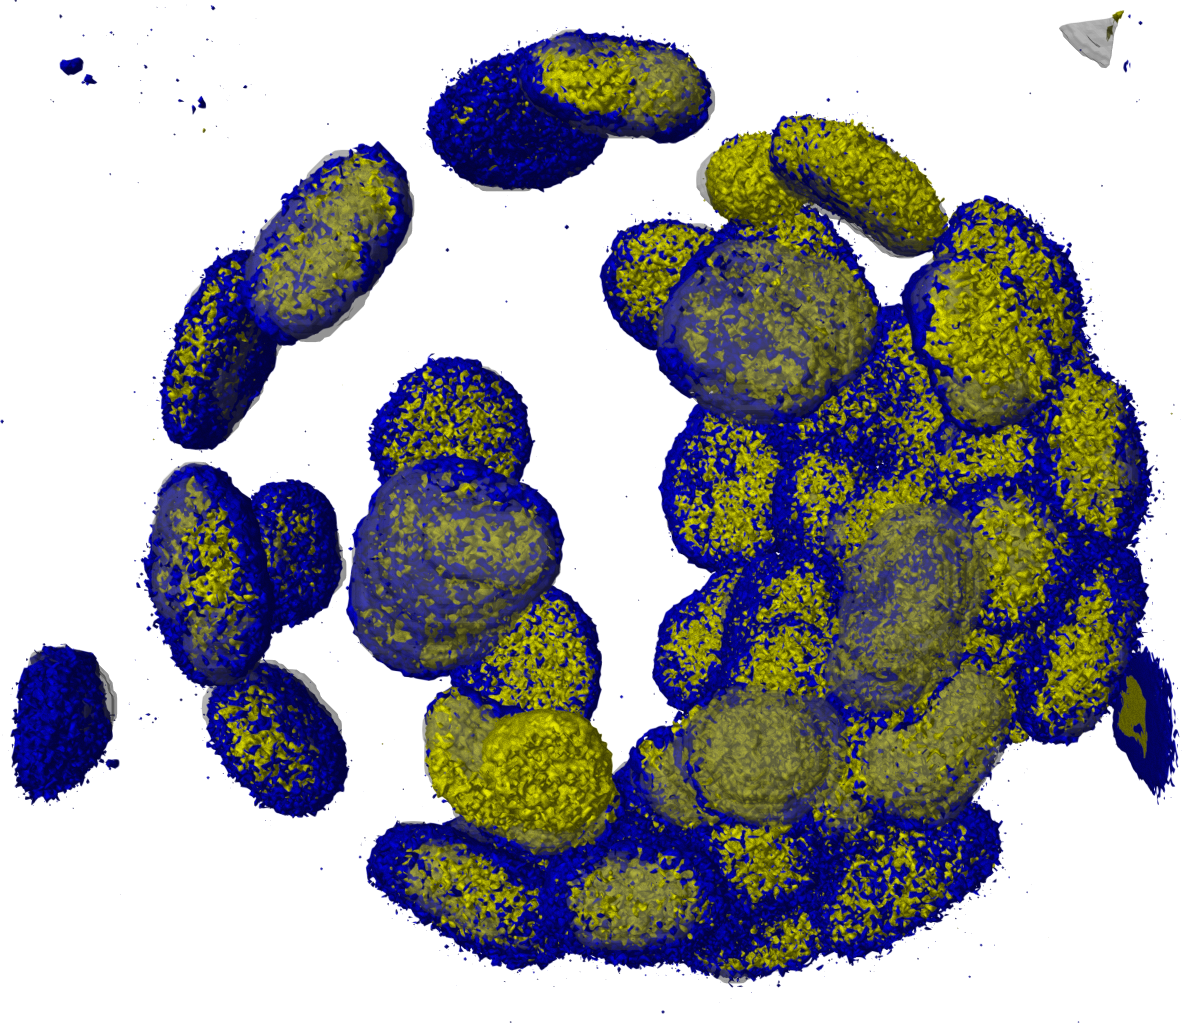
\includegraphics[height=0.5\textheight,keepaspectratio]{images/idr-6001240-mvsx.png}}
  \end{figure}  
  \textbf{Improvements:}
  \begin{itemize}
    \item \alert{Fixed missing volumes, restored color annotations}
    \item Corrected author-defined contour levels
    \item Proper isosurface capping
  \end{itemize}
\end{frame}

\begin{frame}{Conversion Library --- Improvements}
  \begin{figure}
    \centering
    \subfigure[CVSX]{
\includegraphics[height=0.5\textheight,keepaspectratio]{images/contour-missing.png}}
    \hspace{1cm}
    \subfigure[MVSX]{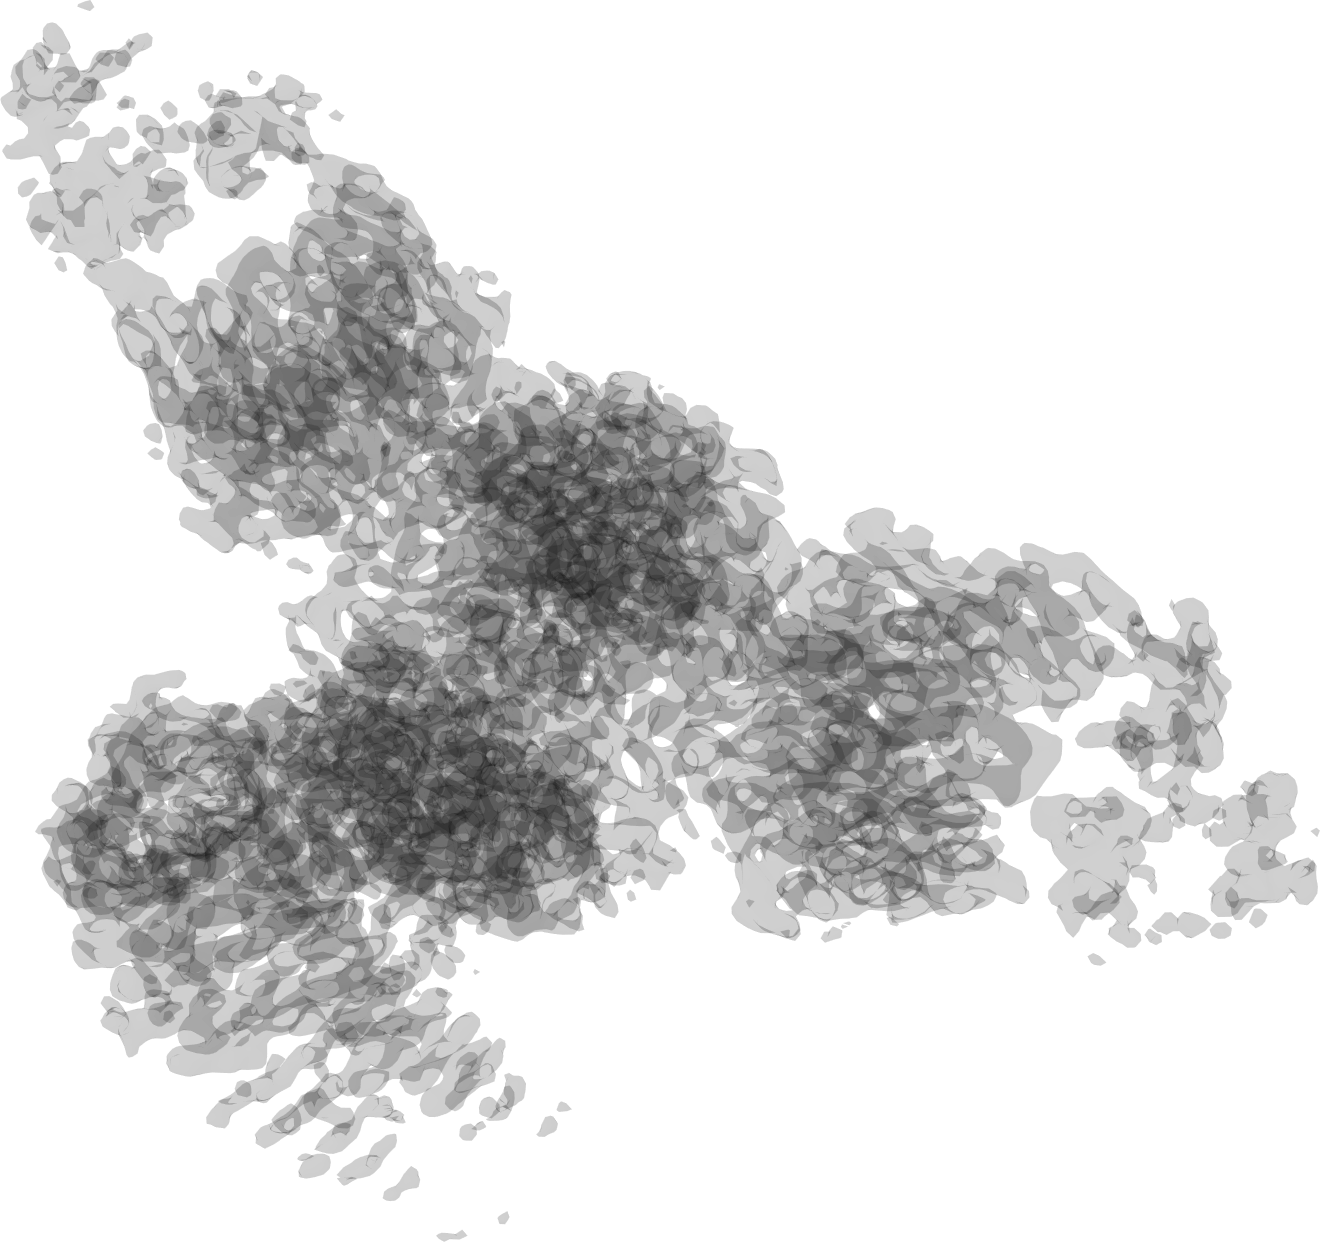
\includegraphics[height=0.5\textheight,keepaspectratio]{images/contour-present.png}}
  \end{figure}  
  \textbf{Improvements:}
  \begin{itemize}
    \item Fixed missing volumes, restored color annotations
    \item \alert{Corrected author-defined contour levels}
    \item Proper isosurface capping
  \end{itemize}
\end{frame}

\begin{frame}{Conversion Library --- Improvements}
  \begin{figure}
    \centering
    \subfigure[CVSX]{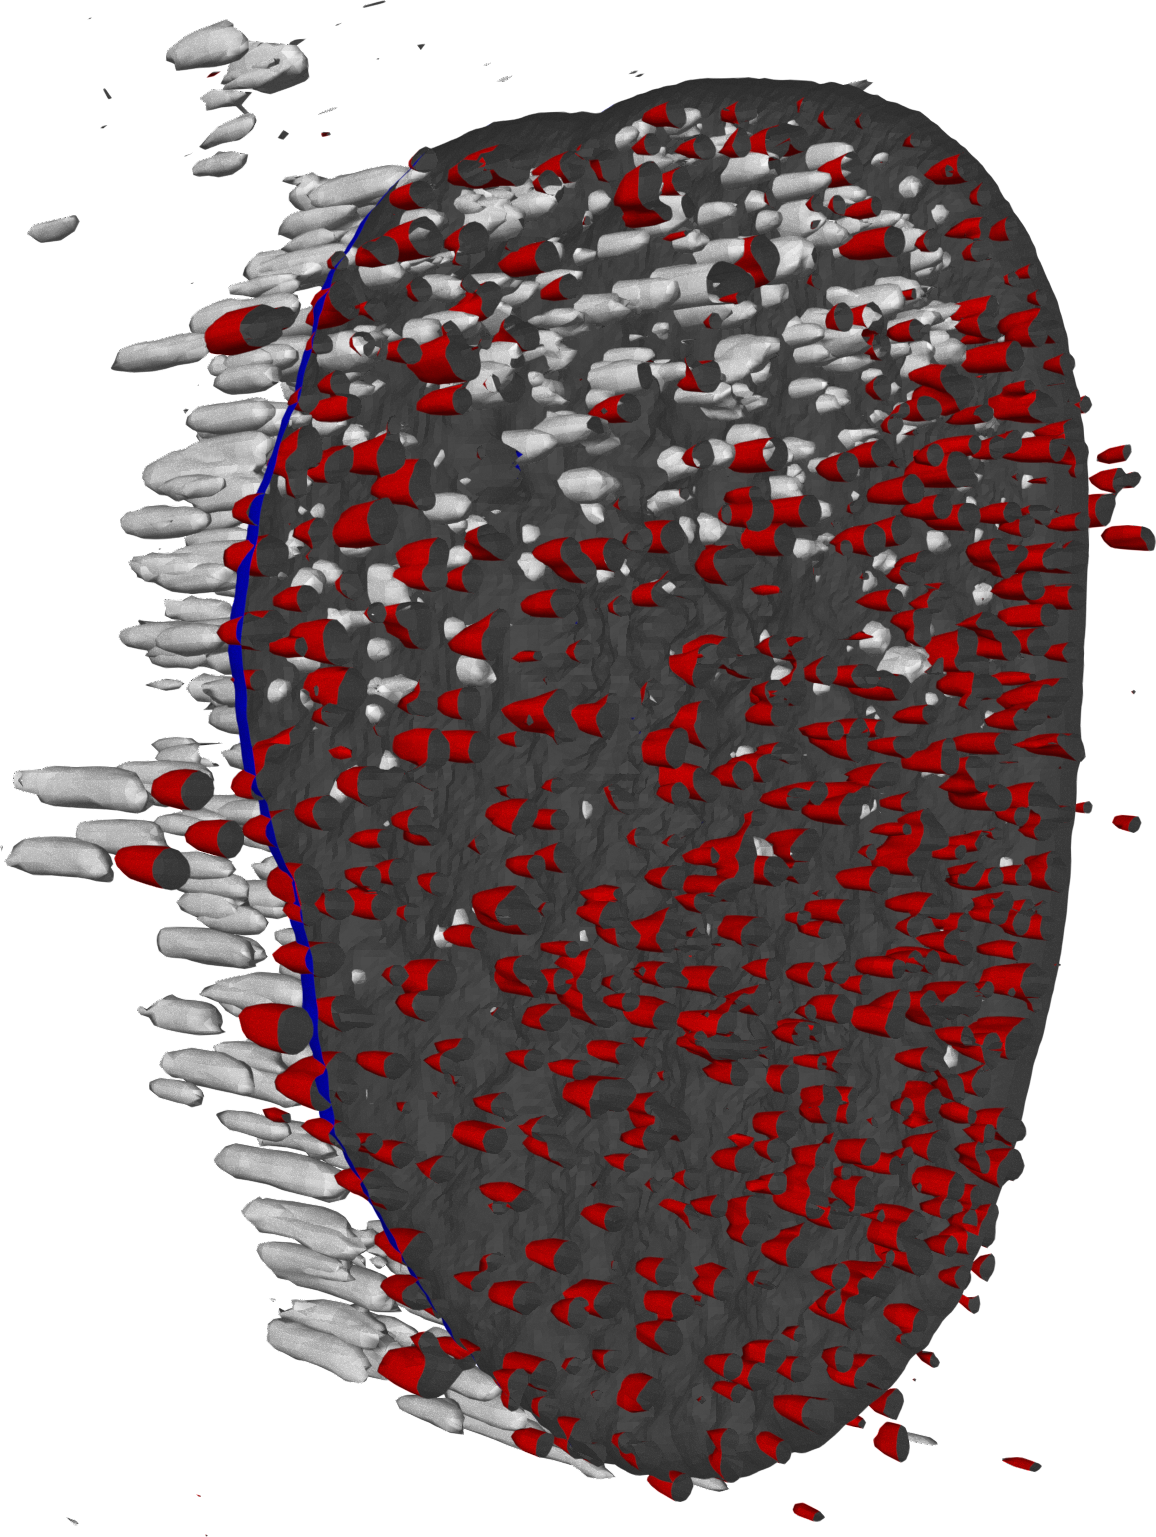
\includegraphics[height=0.5\textheight,keepaspectratio]{images/missing-face-cvsx.png}}
    \hspace{1cm}
    \subfigure[MVSX]{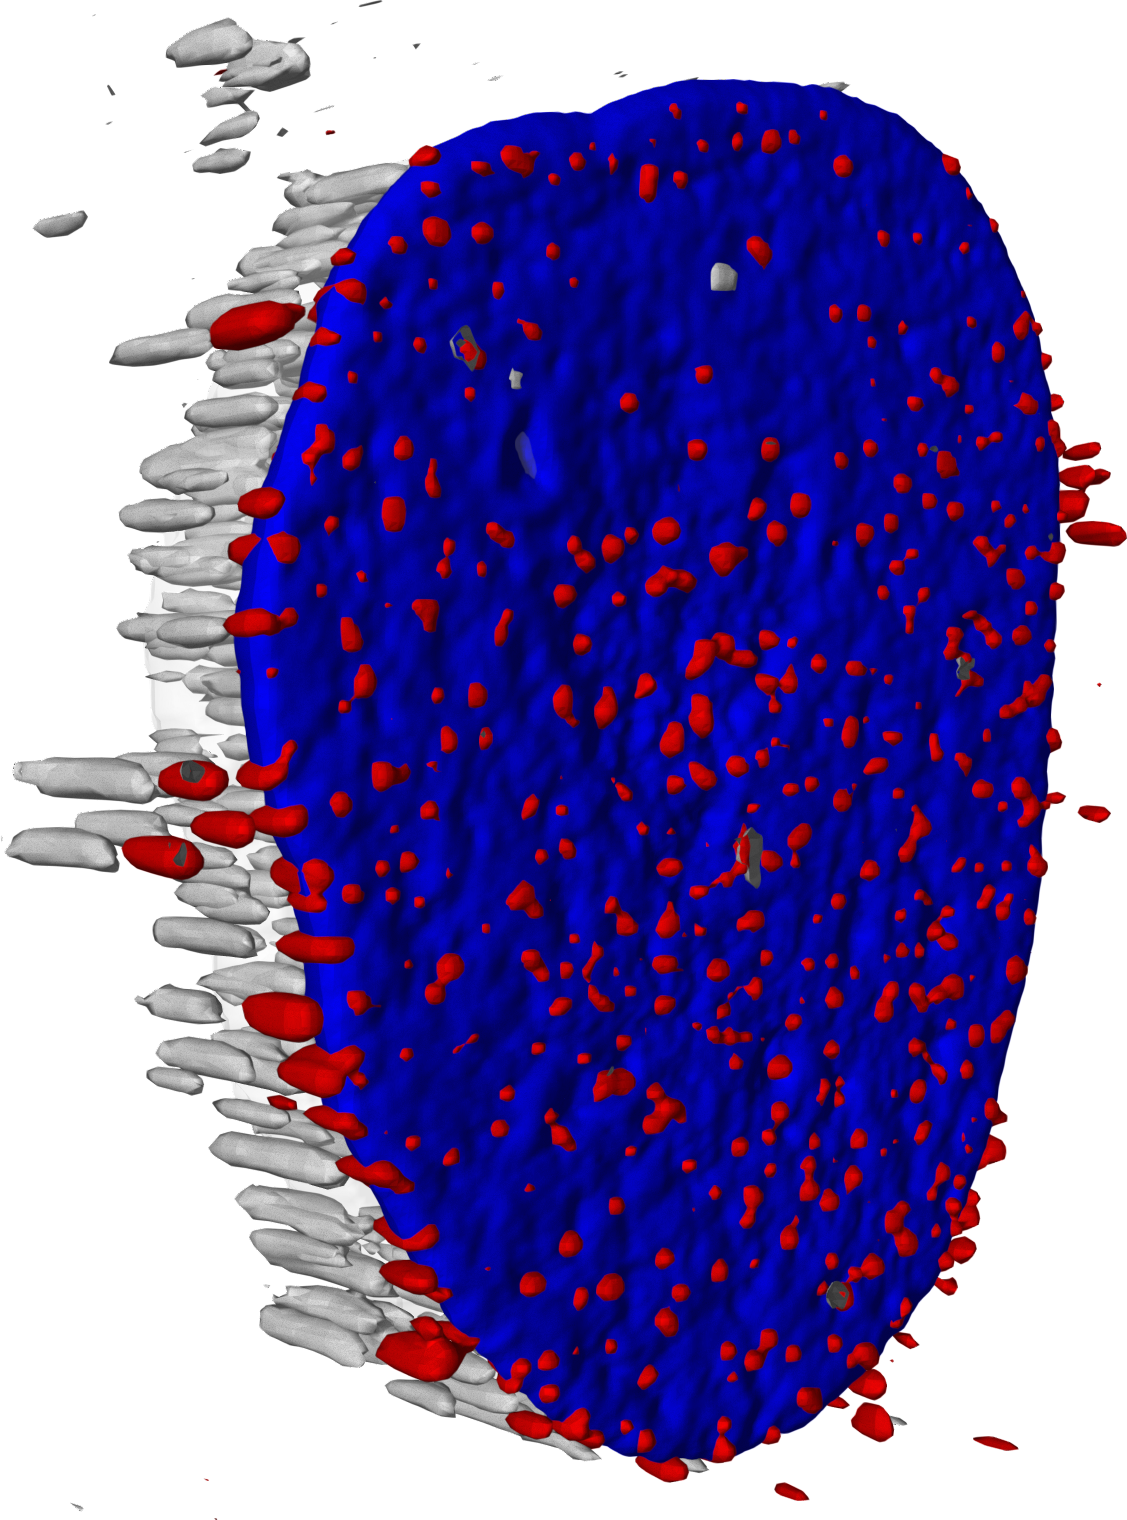
\includegraphics[height=0.5\textheight,keepaspectratio]{images/missing-face-mvsx.png}}
  \end{figure}  
  \textbf{Improvements:}
  \begin{itemize}
    \item Fixed missing volumes, restored color annotations
    \item Corrected author-defined contour levels
    \item \alert{Proper isosurface capping}
  \end{itemize}
\end{frame}

\begin{frame}{Web Application}
  \begin{itemize}
    \item The library is a CLI tool; biologists need a GUI
    \item Interactively update annotations
    \item Collaboration
  \end{itemize}
\end{frame}

\begin{frame}{Web Application --- Implementation}
  \textbf{Architecture:}
  \begin{itemize}
    \item \textbf{Frontend:} React
    \item \textbf{Backend:} FastAPI
    \item \textbf{Storage:} PostgreSQL + MinIO
    \item \textbf{Auth:} e-INFRA AAI 
  \end{itemize}
  \textbf{Infrastructure:}
  \begin{itemize}
    \item Containerized with Docker
    \item Deployed on CERIT-SC Kubernetes cluster
    \item Helm charts for configuration management
    \item CI/CD pipeline via GitHub Actions
  \end{itemize}
\end{frame}

\begin{frame}{Web Application --- Results}
  \begin{figure}
    \includegraphics[height=0.8\textheight,keepaspectratio]{./images/entry-preview.png}
  \end{figure}
\end{frame}

\begin{frame}{Conclusion}
  \begin{itemize}
    \item Replaced the Mol* VS client with MolViewSpec
    \item Conversion library for data migration
    \item Web application for visualizing and annotating
    \item Contributed to a paper \footnote{A. Chareshneu, A. Cantara, \textbf{D. Tichý}, and D. Sehnal. ``Visualizing Volumetric and Segmentation Data using Mol* Volumes \& Segmentations 2.0''. In: \textit{Current Protocols} (2024).}
  \end{itemize}
\end{frame}

\appendix

\section{Otázky oponenta}

\subsection[Otázka 1]{Otázka 1}

\begin{frame}
  \begin{block}{Otázka oponenta 1}
    Narazil jste na nějakou vlastnost nebo typ dat z formátu CVSX, kterou nebylo možno převést do nových formátů MVSX a MVStory?
  \end{block}
  \begin{itemize}
    \item Ano, MolViewSpec nemá zatím přímou podporu pro segmentace
  \end{itemize}
\end{frame}

\subsection[Otázka 2]{Otázka 2}

\begin{frame}
  \begin{block}{Otázka oponenta 2}
    Je nějaký limit velikosti dat, nad který není vaše webová aplikace schopna data zobrazit?
  \end{block}
  \begin{itemize}
    \item Ano, velikost dat je omezena možnostmi Mol*
    \item Největší testovací dataset 500 MB
  \end{itemize}
\end{frame}

\subsection[Otázka 3]{Otázka 3}

\begin{frame}
  \begin{block}{Otázka oponenta 3}
    Jak by bylo možno odstranit drobné vizuální odchylky v renderování, které zmiňujete v sekci 3.4.4?
  \end{block}
  \begin{itemize}
    \item Ano, stačí porovnat verze kódu pro renderování
    \begin{itemize}
      \item Mol* VS - v4.3.0
      \item Mol* - v5.6.1
    \end{itemize}
  \end{itemize}
\end{frame}

\section{Bonus slides}

\subsection{Visual deviations}

\begin{frame}
  \begin{figure}
    \centering
    \subfigure[CVSX]{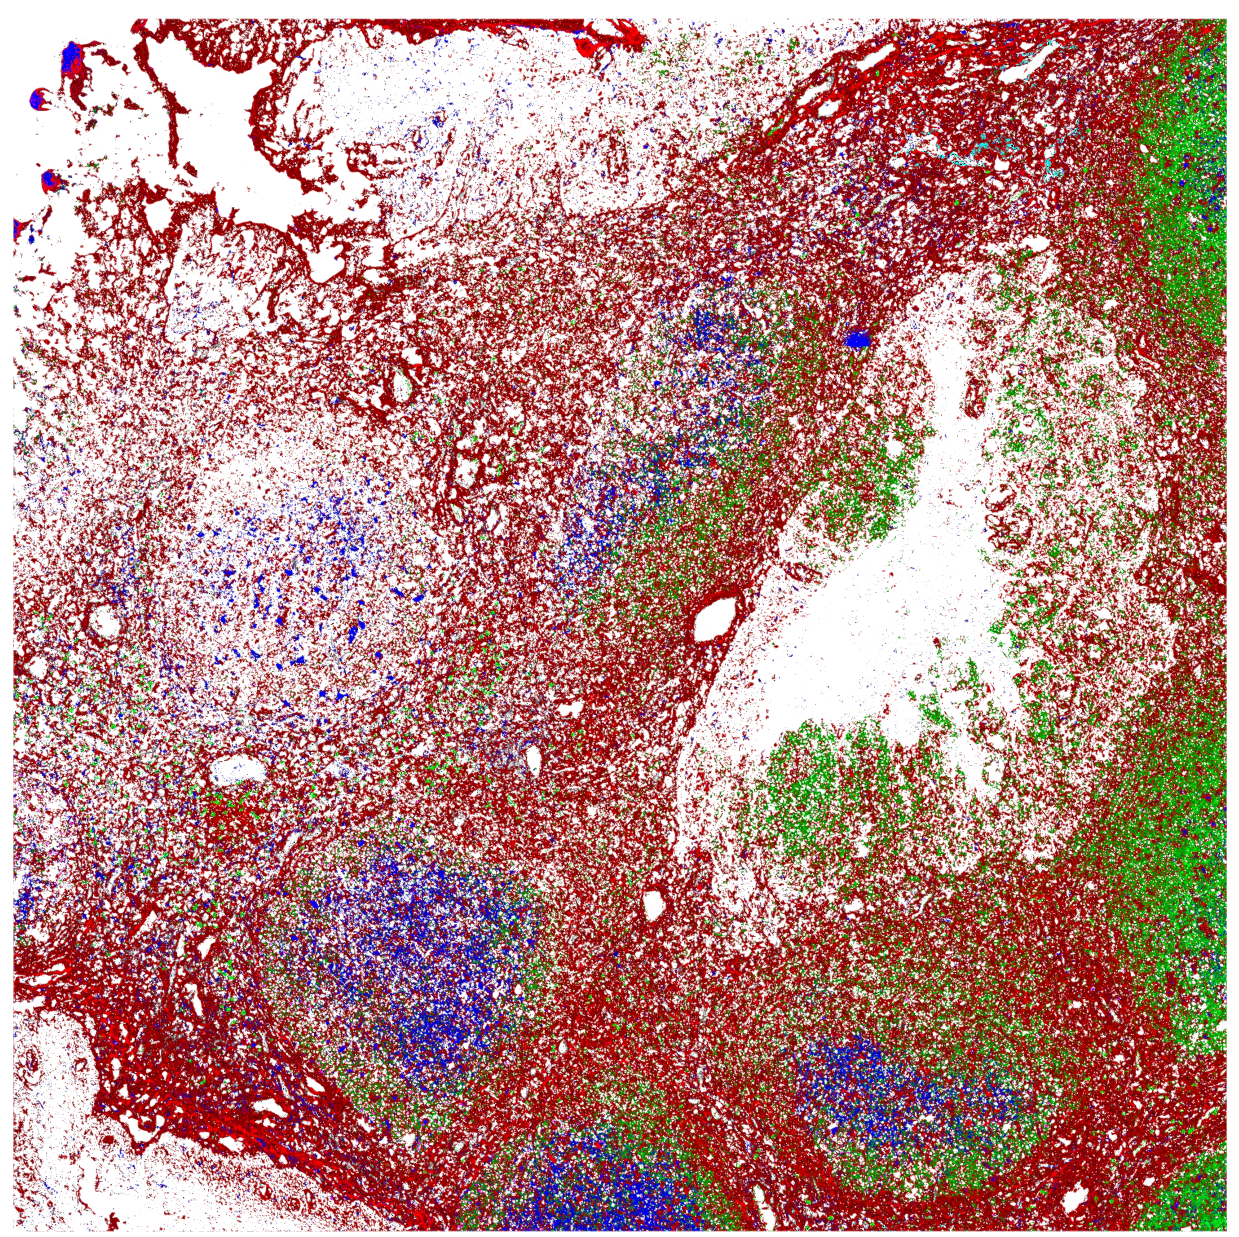
\includegraphics[height=0.4\textheight,keepaspectratio]{images/cvsx-slice.png}}
    \hspace{1cm}
    \subfigure[MVSX]{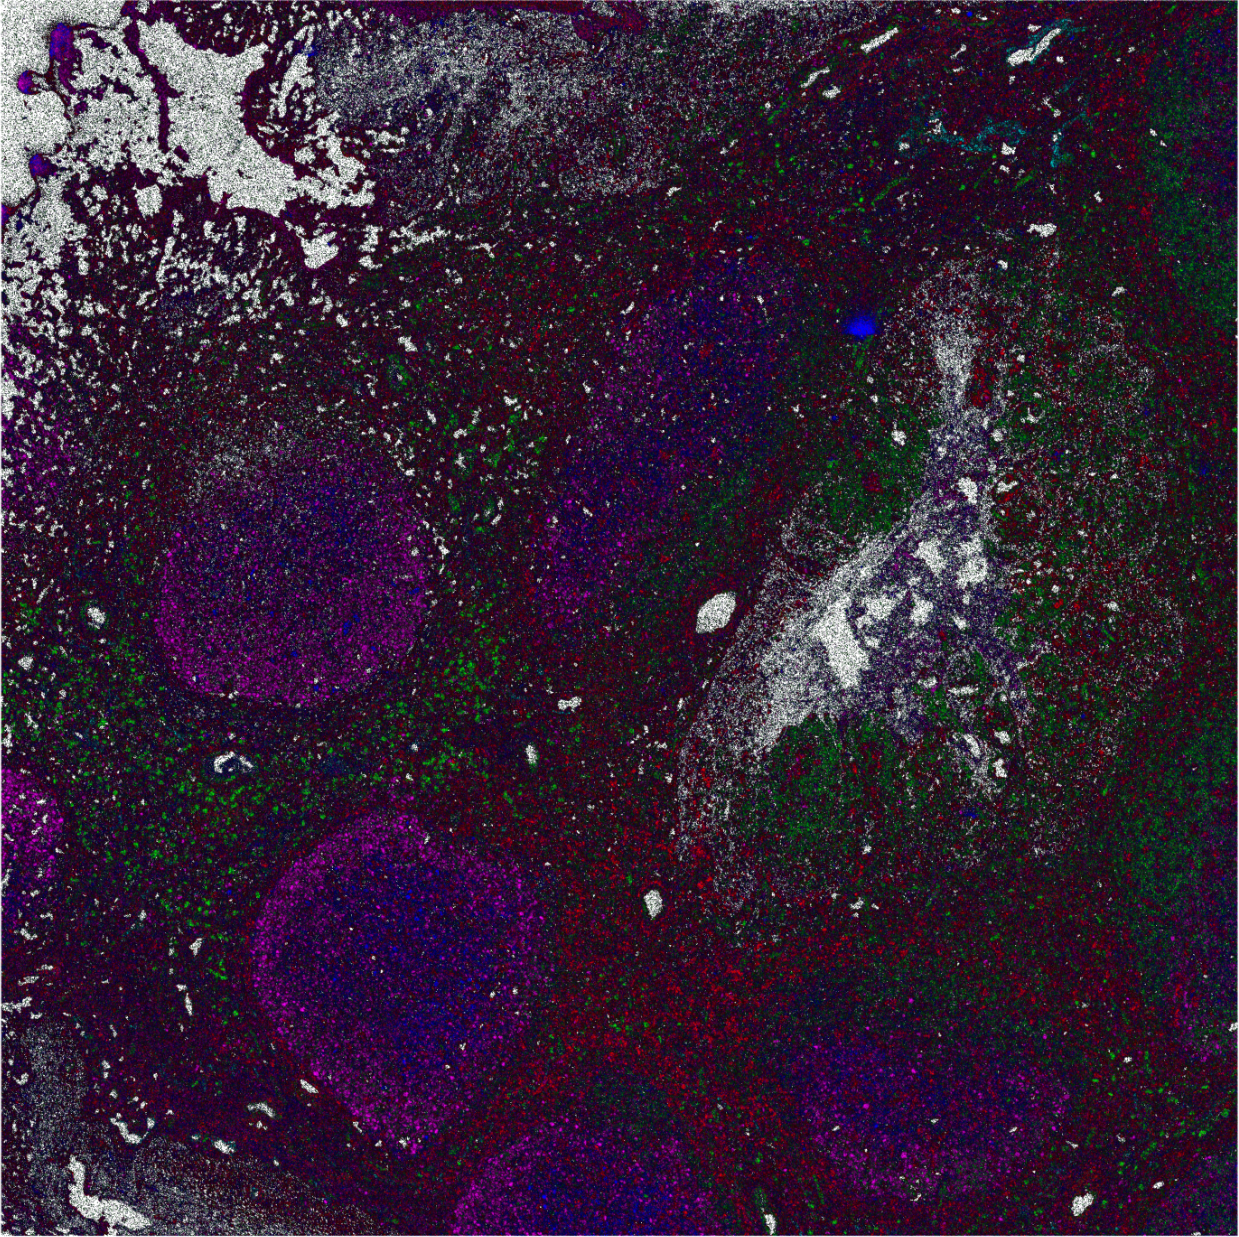
\includegraphics[height=0.4\textheight,keepaspectratio]{images/mvsx-slice.png}}
    \subfigure[Vizarr]{\includegraphics[height=0.4\textheight,keepaspectratio]{images/original.png}}
  \end{figure}  
\end{frame}

\makeoutro
\addtocounter{framenumber}{-1}

\end{document}
